在不同的内核形式之间进行选择,很大程度上取决于个人偏好,并且很受到以前使用其他并行编程模型和语言经验的影响。\par

选择内核形式的另一个原因是,公开内核所需的功能。不幸的是,在开发开始之前很难确定需要哪些功能——特别是当我们不熟悉不同的内核形式,以及它们与各种类是如何交互时。\par

为了帮助读者们进行选择,我们根据自己的经验构建了两个指南。读者可以参考这些经验法则,但最好的方法是选择不同的内核形式进行编写,对不同的方式进行测试和了解,从而在开发应用程序时选择最合适的内核形式和开发方式。\par

第一个指南是如图4-26所示的流程图:\par

\begin{itemize}
	\item 是否有并行编程的经验
	\item 是从头编写新代码,还是移植用现有的并行程序
	\item 是包含嵌套的并行,还是在内核函数的不同实例之间重用数据
	\item 用SYCL编写新内核是为了最大化性能,还是为了提高代码的可移植性,使用比底层的语言更高效的方式表示并行性
\end{itemize}

\hspace*{\fill} \par %插入空行
图4-26 选择正确的内核形式
\begin{center}
	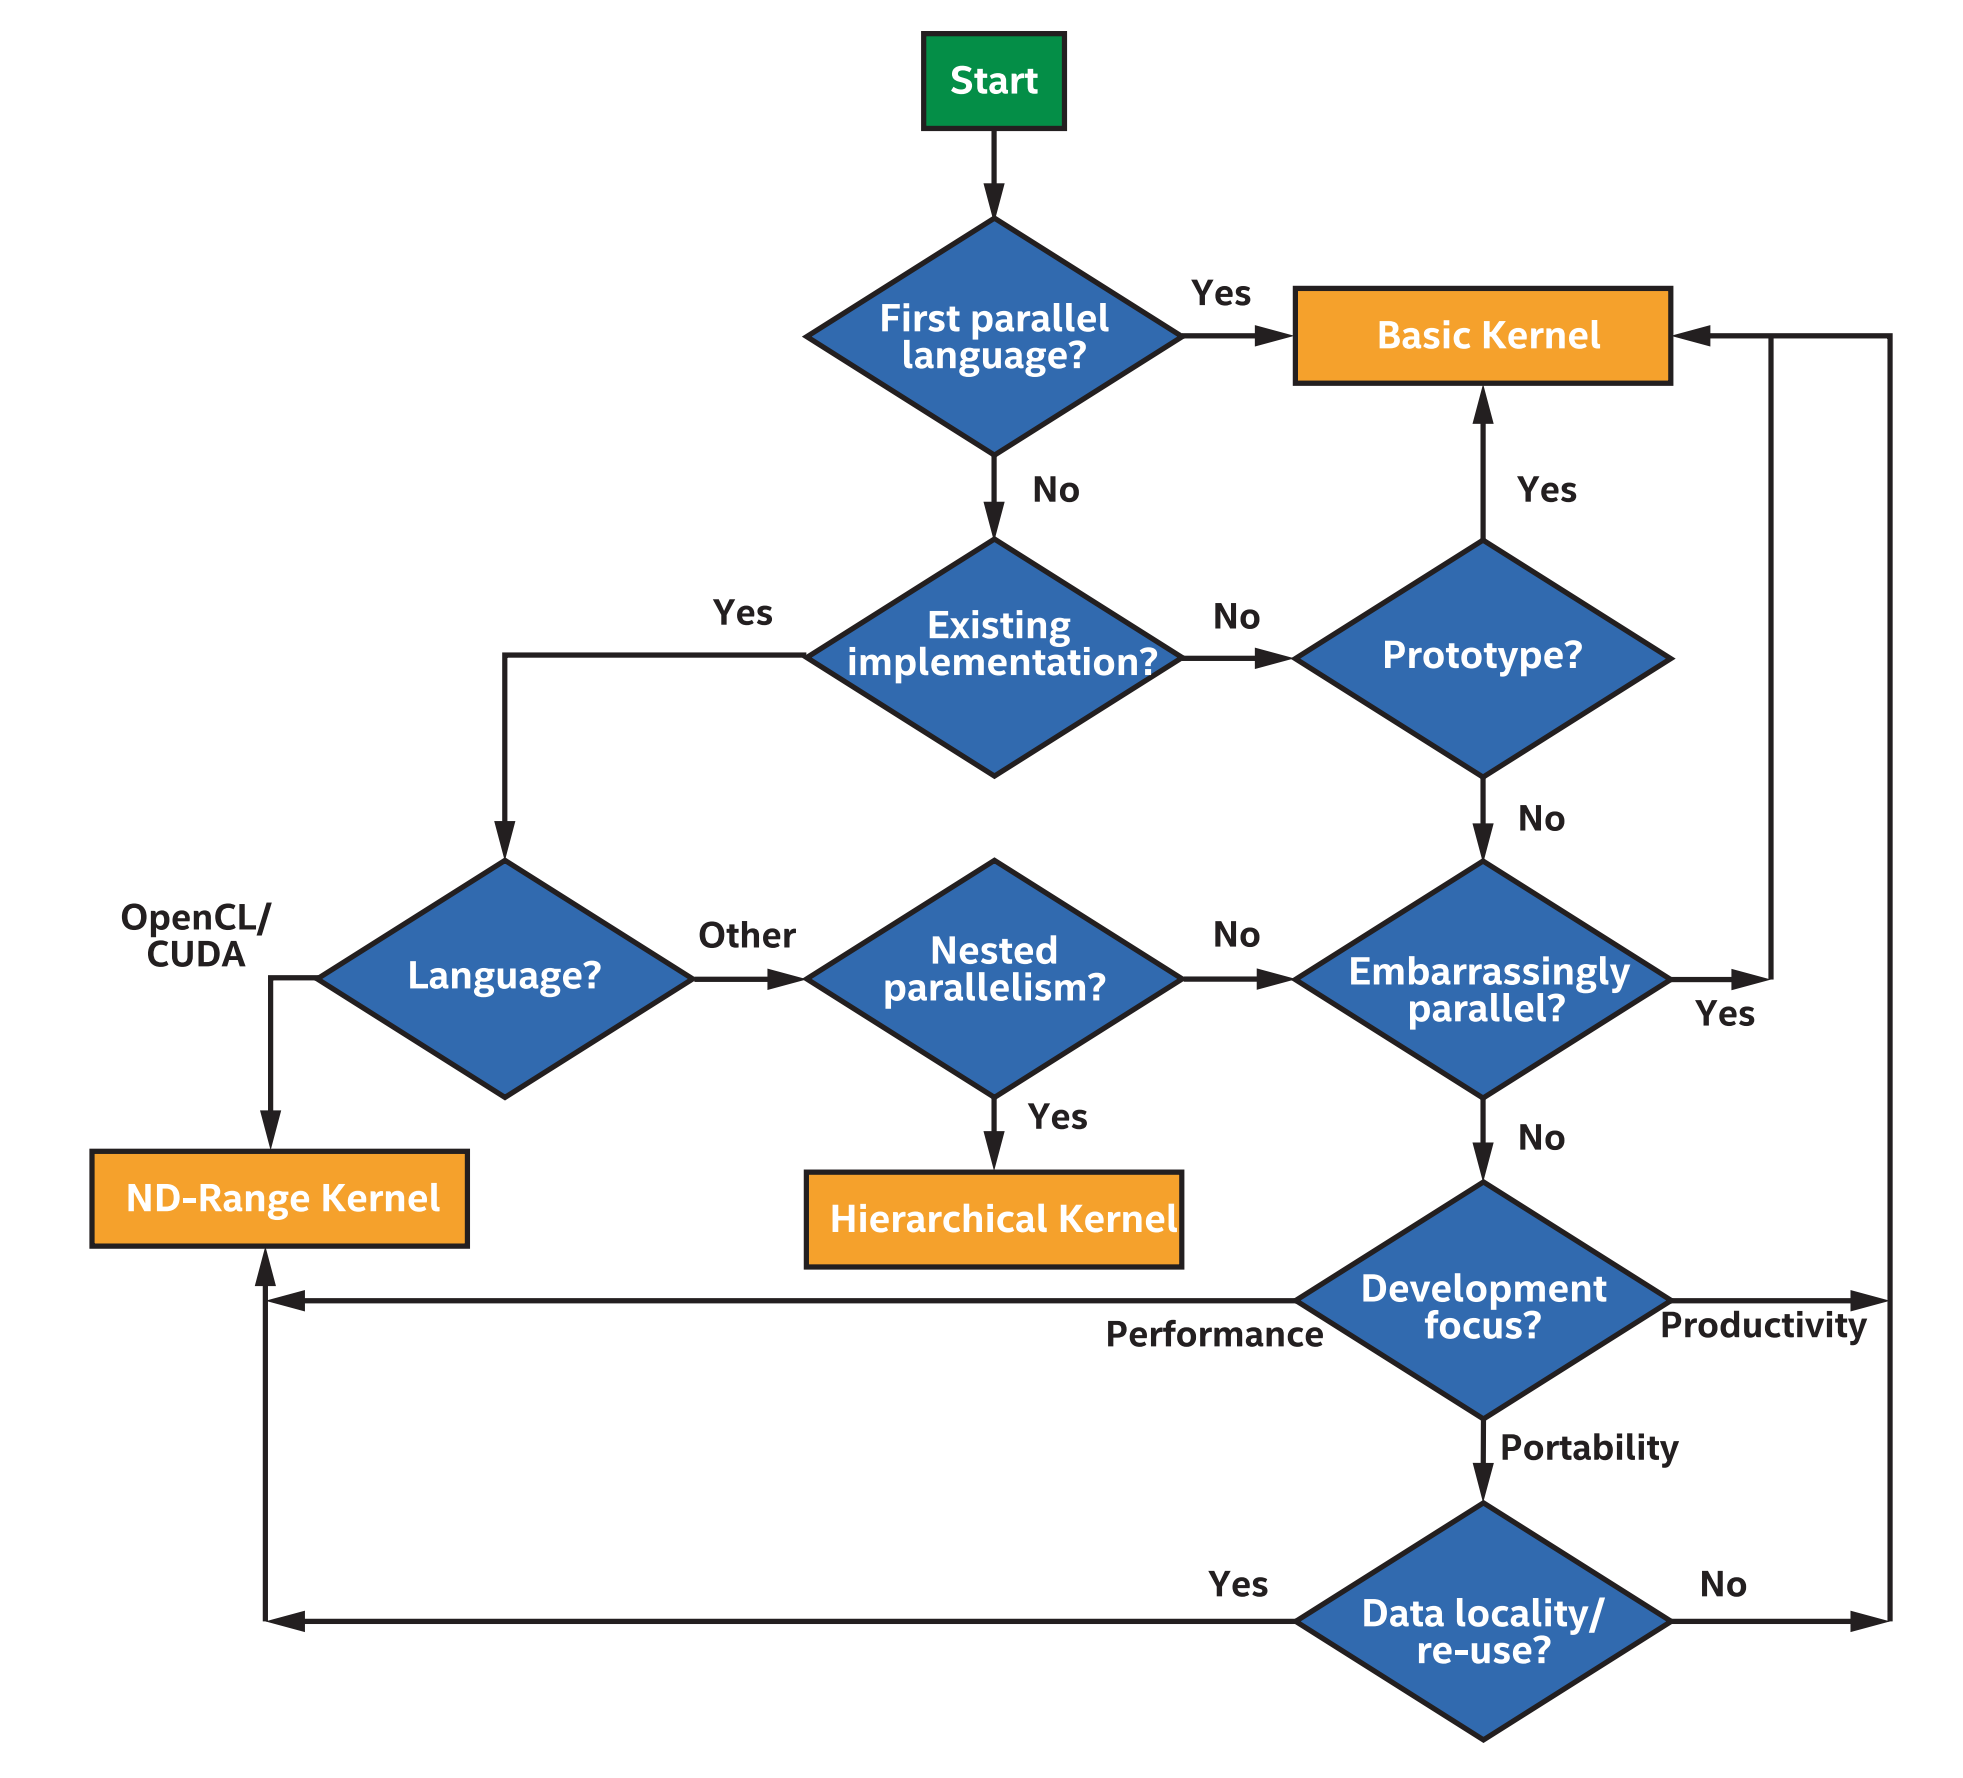
\includegraphics[width=0.8\textwidth]{content/chapter-4/images/7}
\end{center}

第二个指南是图4-27中的表格,总结了每种内核形式公开的功能。值得注意的是,这个表反映了DPC++在本书出版时的状态,随着语言的发展,每个内核形式可用的特性会发生变化。预计基本趋势将保持不变:基本的数据并行内核不会公开位置感知特性,显式的ND-Range内核会公开所有支持性能的特性,分层内核在公开特性方面会落后于显式的ND-Range内核,但是对这些特性的表达将使用更高层的抽象。\par

\hspace*{\fill} \par %插入空行
图4-27 每种内核形式的特性
\begin{table}[H]
	\begin{tabular}{|l|c|c|c|}
		\hline
		\textbf{特性}                           & \multicolumn{1}{l|}{\textbf{基本内核}} & \multicolumn{1}{l|}{\textbf{ND-Range内核}} & \multicolumn{1}{l|}{\textbf{层次内核}} \\ \hline
		\textbf{工作组本地内存}           & No                                         & Yes                                           & Yes                                              \\ \hline
		\textbf{工作组栅栏}               & No                                         & Yes                                           & Yes                                              \\ \hline
		\textbf{子工作组}                        & No                                         & Yes                                           & No                                               \\ \hline
		\textbf{工作组函数(比如:scan,reduce)} & No                                         & Yes                                           & No                                               \\ \hline
	\end{tabular}
\end{table}




